\documentclass[tikz,border=4pt]{standalone}
\usepackage{amsmath,amssymb}
\usetikzlibrary{arrows.meta,positioning,calc}
\begin{document}
    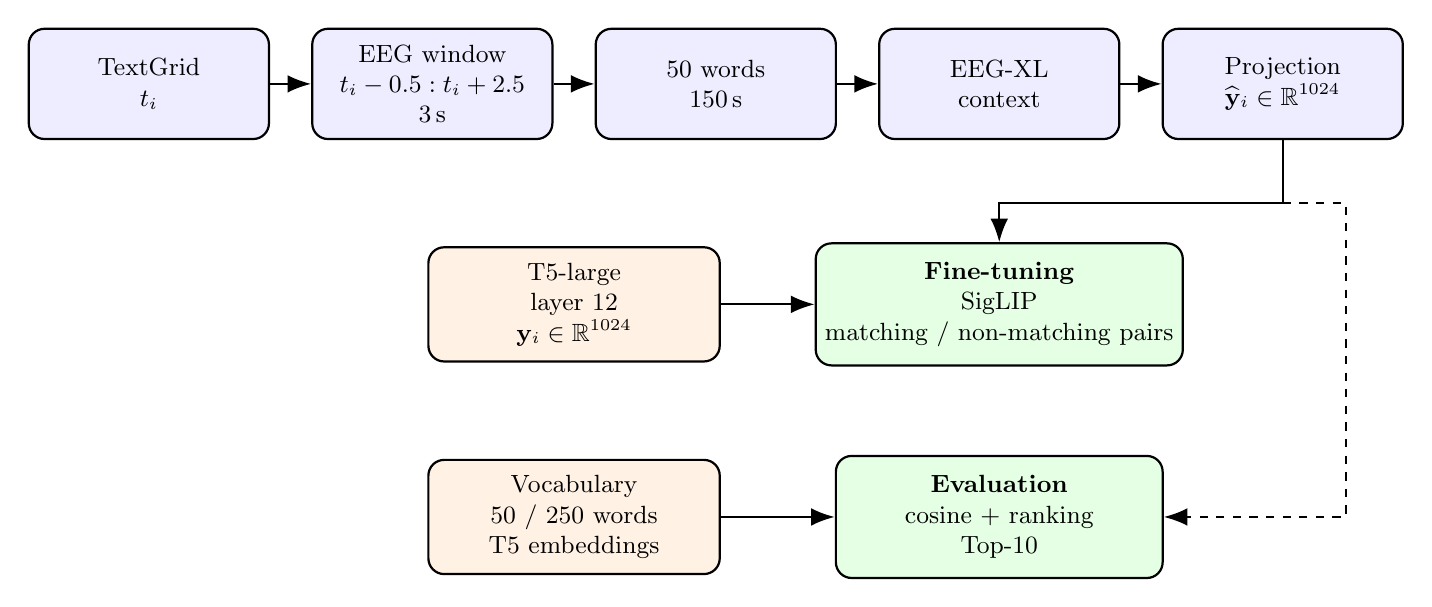
\begin{tikzpicture}[
        font=\small,
        arrow/.style={-{Latex[length=3mm]}, thick},
        box/.style={draw, rounded corners=2mm, minimum width=3.05cm,
                   minimum height=1.4cm, align=center, thick, fill=blue!7},
        language/.style={draw, rounded corners=2mm, minimum width=3.7cm,
                        minimum height=1.45cm, align=center, thick, fill=orange!10},
        train/.style={draw, rounded corners=2mm, minimum width=4.15cm,
                     minimum height=1.55cm, align=center, thick, fill=green!10},
        note/.style={font=\footnotesize, align=center}
    ]
        \node[box] (textgrid) at (0,3.6) {TextGrid\\$t_i$};
        \node[box] (epoch) at (3.6,3.6) {EEG window\\$t_i-0.5:t_i+2.5$\\$3\,\mathrm{s}$};
        \node[box] (sequence) at (7.2,3.6) {50 words\\$150\,\mathrm{s}$};
        \node[box] (encoder) at (10.8,3.6) {EEG-XL\\context};
        \node[box] (project) at (14.4,3.6) {Projection\\$\widehat{\mathbf{y}}_i\in\mathbb{R}^{1024}$};

        \draw[arrow] (textgrid) -- (epoch);
        \draw[arrow] (epoch) -- (sequence);
        \draw[arrow] (sequence) -- (encoder);
        \draw[arrow] (encoder) -- (project);

        \node[language] (t5) at (5.4,0.8) {T5-large\\layer 12\\$\mathbf{y}_i\in\mathbb{R}^{1024}$};
        \node[train] (siglip) at (10.8,0.8) {\textbf{Fine-tuning}\\SigLIP\\matching / non-matching pairs};

        \node[language] (vocab) at (5.4,-1.9) {Vocabulary\\50 / 250 words\\T5 embeddings};
        \node[train] (retrieval) at (10.8,-1.9) {\textbf{Evaluation}\\cosine + ranking\\Top-10};

        \draw[arrow] (t5) -- (siglip);
        \coordinate (split) at ($(project.south)+(0,-8mm)$);
        \draw[thick] (project.south) -- (split);
        \draw[arrow] (split) -| (siglip.north);
        \draw[arrow] (vocab) -- (retrieval);
        \draw[arrow, dashed] (split) -- ++(8mm,0) |- (retrieval.east);
    \end{tikzpicture}
\end{document}
